\begin{multicols}{2}
\part*{\textbf{Квадрат Пирсона}}
\emph{А.П. Азия, И.М. Вольпер}\large{}
\vspace{4cm}
\par
В "Занимательной алгебре" Я. И. Перельмана есть любопытная задача под названием "В парикмахерской". В этой задаче автор рассказывает, что, заглянув однажды в парикмахерскую, он увидел, как мастера пытались безуспешно приготовить 12-процентный раствор перекиси водорода из двух имеющихся в наличии растворов - трёх и тридцатипроцентного*).
\par
Задача, описанная Перельманом, встречается не только в парикмахерских.
\par
Например, для зарядки аккумуляторов бывает необходимо приготовить электролит, которй должен содержать 24\% серной кислоты из двух растворов с содержанием 92\% и 10\% серной кислоты. На консервных заводах возникает необходимость приготовления 6\%-ного уксуса для маринада из двух партий уксуса разной крепости: 3\% и 10\%, и т.д.
\par
Для решения подобных задач удобно пользоваться "квадратом Пирсона". Вот как это делается. Рисуют квадрат и проводят две диагонали(рис. 1). В левом верхнем углу проставляют больший показатель крепости исходных веществ(а), а в нижнем углу - второй показатель (b), а на пересечении диагоналей записывают требуемый показатель смеси(с). Затем производят вычитание по первой диагонали (a - c) и находят количество
\hline
*) Напомним, что содержанием вещества в растворе называется отношение массы этого вещества в "чистом виде" к массе раствора.
\columnbreak
второй части смеси(у). Из центра производят вычитание по второй диагонали (с - b) и находят количество первой части смеси(х). Значения х и у записывают по одной линии с показателями. На х частей первого вещества надо взять у часей второго вещества, тогда получится смесь с показателем с.
\begin{minipage}[h]{0.49\linewidth}
\center{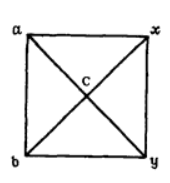
\includegraphics[width=0.7\linewidth]{image1.png}} \\
\caption{рис. 1}
\end{minipage}
\hfill
\begin{minipage}[h]{0.49\linewidth}
\center{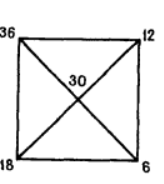
\includegraphics[width=0.7\linewidth]{image2.png}} \\
\caption{рис. 2}
\end{minipage}


\par
Пусть, например, имеются две партии сливок: одна содержит 36\% жира, а другая - 18\%. Требуется определить, сколько надо взять тех и других сливок, чтобы получить смесь с количеством жира 30\%. Решаем по изложенному выше способу(рис. 2) и получаем
\begin{equation*}
    \begin{split}
        y=a-c=36-30=6&
        &x=c-b=30-18=12
    \end{split}
\end{equation*}




то есть на 6 массовых частей второй партии сливок надо взять 12 частей первой.
\par
Этот способ основан на специфическом виде количества получаемой смеси, оно равно разности показателей исходных веществ. Такое допущение вполне возможно, так как нас интересут не абсолютные величины, а относительные количества двух частей смеси.
\par 
В самом деле, мы получаем $x+y=(c-b)+(a+c)=a-b$ частей смеси. "Чистого" вещества в ней будет \begin{equation*}
    \frac{x \cdot a}{100}+\frac{y \cdot b}{100}=\frac{(c-b)\cdot a+ (a-c)b}{100}=\frac{ac-bc}{100}
\end{equation*}
частей, а крепость смеси будет равна $\frac{ac-bc}{100(a-b)}=\frac{c}{100}$, то есть с \%.
\end{multicols}

\newpage
исходники: git